\section{Decisiones técnicas}
    En esta sección se plantean las herramientas y tecnologías que se van a utilizar para llevar a cabo el desarrollo del proyecto, justificando cada una de ellas.
    
    \subsection{Frontend} 
        Para programar el frontend de la aplicación web para empleados se utilizará HTML, CSS y JavaScript. 
        Se usará también Jinja2, un motor de plantillas integrado con Flask que permite generar HTML de manera dinámica.
     
    \subsection{Backend}
        Para programar la lógica del backend de la aplicación se utilizará Python. 
        Servirá de conexión entre Dialogflow, la base de datos y la aplicación web. 
            
        Se utilizará este lenguaje por su flexibilidad y facilidad para integrar todos los servicios. Algunas de las librerías que se emplearán son:
        \begin{itemize}
            \item Flask: framework web para crear aplicaciones web. Se utilizará para desarrollar el backend de la aplicación.
            \item SQLAlchemy: sirve para interactuar con la base de datos SQLite de manera sencilla y eficiente.
            \item Discord.py: librería para interactuar con Discord y programar el bot que atenderá las llamadas VoIP.
            \item Google-Cloud-Dialogflow y Google-Cloud-Speech: para interactuar con los servicios de IA de Google Cloud.
            \item Selenium: para automatizar la simulación de los trámites en las webs oficiales.
        \end{itemize}

    \subsection{Base de datos}
        SQLite es el lenguaje elegido para programar la base de datos ya que está integrado con Python y es suficiente para almacenar la información de nuestro sistema simulado. 

    \subsection{Servicios}
        Algunas de las herramientas y servicios externos que se van a utilizar son:
        \begin{itemize}
            \item Google Cloud: se va a utilizar esta plataforma en la nube para alojar los diferentes servicios de inteligencia artificial del proyecto.
                Se prefiere esta opción frente a otras alternativas ya que integra un servicio propio de agentes conversacionales, ofreciendo un plan gratuito suficiente para el desarrollo.
                \begin{itemize}
                    \item Dialogflow ES: es la herramienta de Google Cloud para crear agentes conversacionales capaces de interpretar el lenguaje natural y las intenciones del usuario mediante algoritmos de machine learning. 
                        Se utilizará para definir las intenciones y los flujos de conversación que podrán tener los usuarios con el agente, recopilar la información requerida para los trámites y devolver el audio a reproducir en la llamada.
                        Esta opción es la más adecuada para proyectos pequeños con pocos trámites.
                    \item Goolge Speech-to-Text: servicio de reconocimiento de voz que convierte el audio de las llamadas VoIP en texto para que pueda ser procesado por Dialogflow. 
                        También se implementará un servicio speech-to-text local con Vosk para poder hacer consultas en desarrollo sin gastos de créditos de Google Cloud.
                \end{itemize}
            \item Discord: es una plataforma de comunicación que permite llamadas VoIP, se usará por la facilidad para crear aplicaciones y bots fácilmente programable en python.
                El usuario iniciará una llamada uniéndose a un canal de Discord y el bot comenzará una conversación conectándose con las IA de Google Cloud.
            \item Gitlab: se usará un control de versiones para mantener actualizados todos los cambios en el código y la documentación del proyecto, y poder recuperar cualquier versión ante un imprevisto. 
            \item Ngrok: crea un túnel desde el despliegue local para tener un endpoint público en desarrollo, necesario para comunicar el backend con Dialogflow. 
                Es una herramienta segura que evita los costes de mantener un servidor propio para la implementación del proyecto, manteniéndonos dentro del alcance definido.
        \end{itemize}
    
    \subsection{Documentación}
        Para la documentación del proyecto se utilizarán las siguientes herramientas:
        \begin{itemize}
            \item Figma: herramienta de diseño para crear los mockups de la interfaz de usuario.
            \item Draw.io: es una herramienta de diseño para crear los diagramas fácilmente para la memoria.
            \item Latex: como sistema de composición de textos para escribir la memoria.
        \end{itemize}

\section{Diseño de la interfaz de usuario}
    En esta sección se muestra el diseño adoptado en la interfaz de la aplicación web destinada a trabajadores de las Administraciones públicas.
    El concepto general de la interfaz se ha centrado en mostrar únicamente la información y funcionalidades necesarias en pantalla, manteniendo un estilo simple y claro que favorece la eficiencia y eficacia en el uso de la aplicación.

    A continuación se presentan los mockups de las páginas principales del sistema.
    En cada prototipo se describen los elementos que lo componen, explicando las funcionalidades que disponen los empleados.

    \begin{figure}[H]
        \centering
        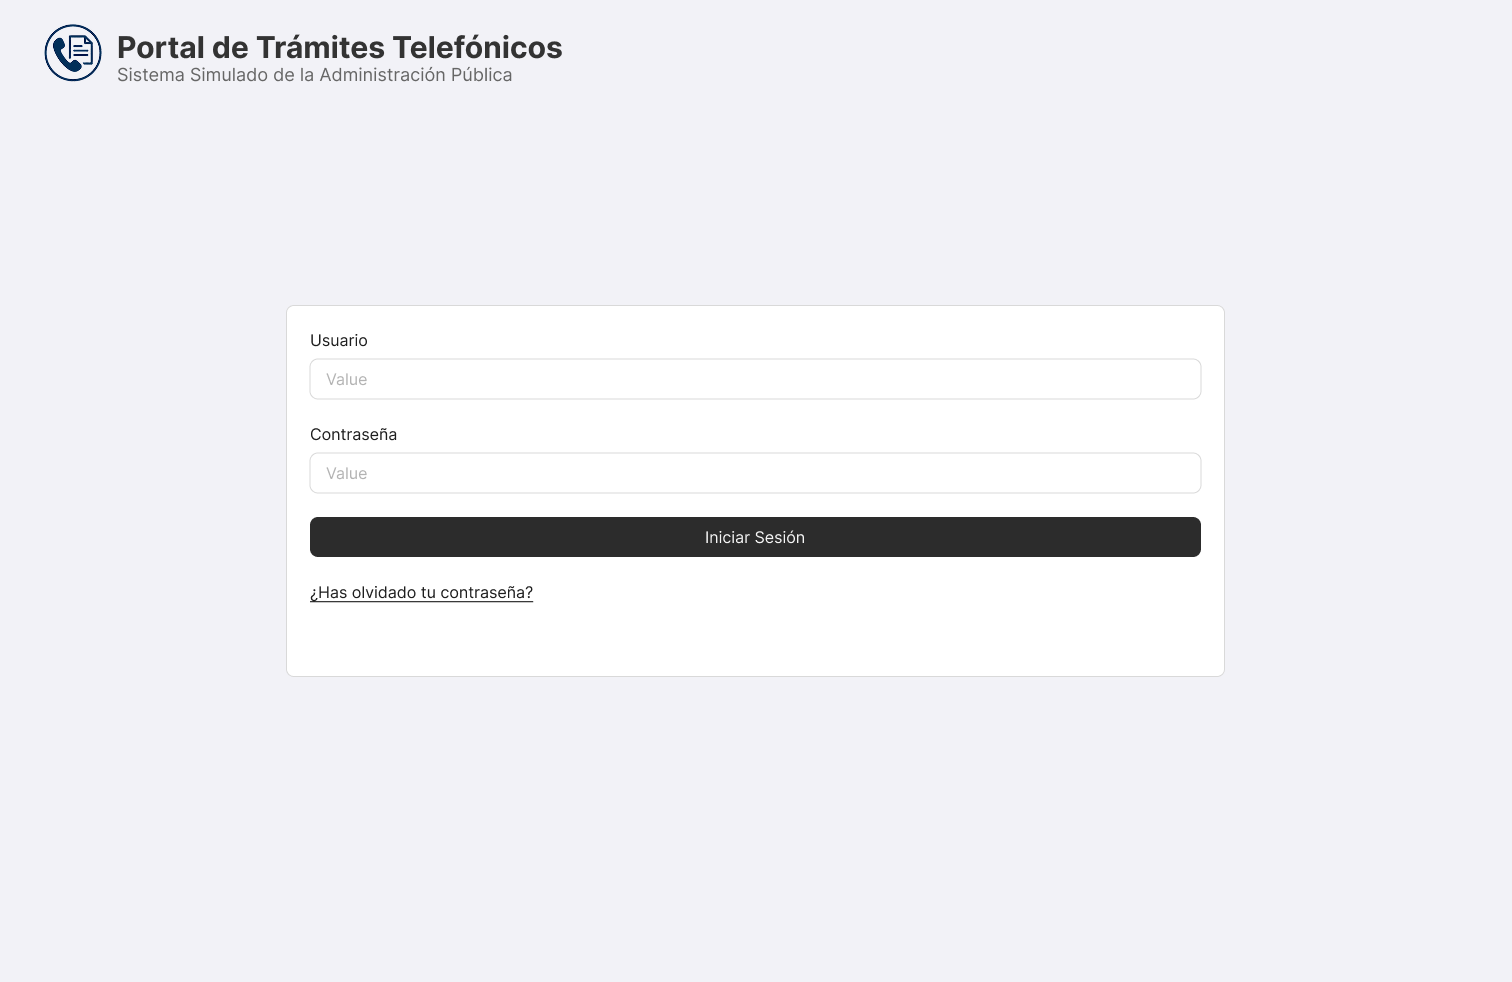
\includegraphics[width=0.8\textwidth]{img/mockups/Login.png}
        \caption{Prototipo visual de la página de login.}
        \label{fig:4.1}
    \end{figure}
    La figura \ref{fig:4.1} muestra la pantalla de inicio de sesión del sistema. 
    Se trata de la página inicial de la aplicación y la única accesible públicamente para usuarios ajenos al sistema.
    Por ello, presenta únicamente un formulario de acceso en la parte central, que permite a los empleados identificarse fácilmente mediante sus credenciales.
        
    Para acceder a cualquier otra página del sistema es necesario autenticarse para garantizar la confidencialidad de la información.

    \begin{figure}[H]
        \centering
        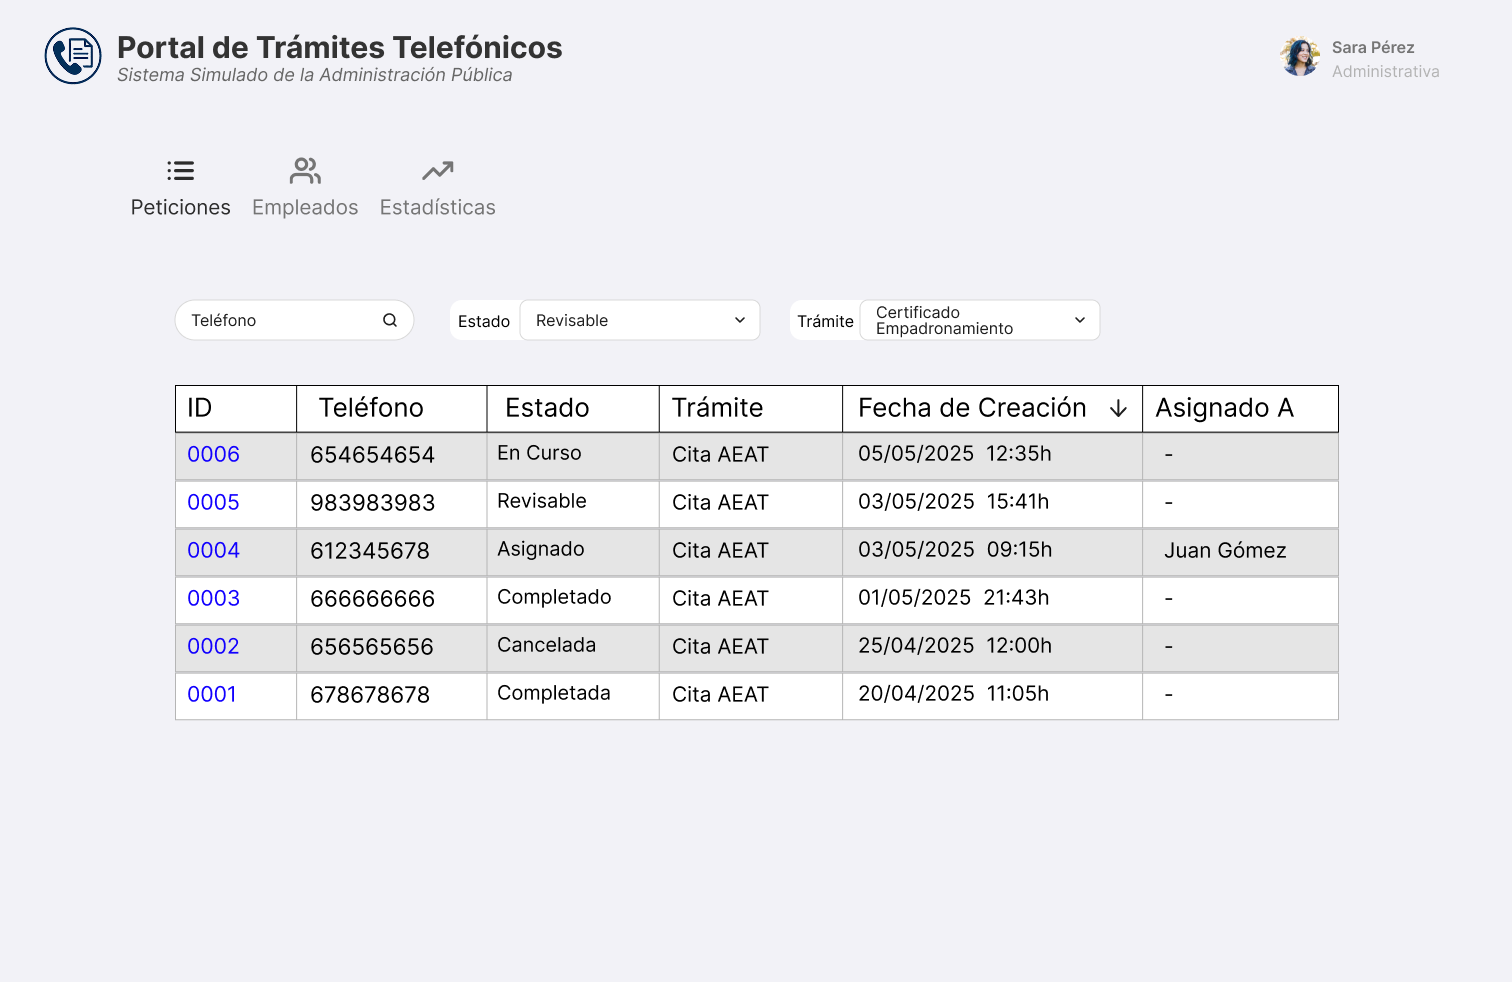
\includegraphics[width=0.8\textwidth]{img/mockups/Peticiones.png}
        \caption{Prototipo visual de la página de peticiones.}
        \label{fig:4.2}
    \end{figure}
    La figura \ref{fig:4.2} muestra un listado con todas las peticiones del sistema. 
    Se trata de la página principal de la aplicación, ya que es visible por todos los empleados.
        
    El componente principal es una tabla con la información básica de cada petición, incluyendo en la parte superior de la tabla una serie de filtros para localizar rápidamente la gestión deseada.
    En cada fila de la tabla se incluye un link, situado en la columna con del ID, para navegar a una página con detalles específicos de cada petición.
    Además, en la parte superior izquierda, debajo del logotipo, se incluye un menú para navegar entre las distintas páginas. 
        
    Por último, todas las páginas incluyen el perfil del empleado identificado en la parte superior derecha. 
    Clicando sobre el perfil se puede navegar hasta la página con detalles del empleado.

    \begin{figure}[H]
        \centering
        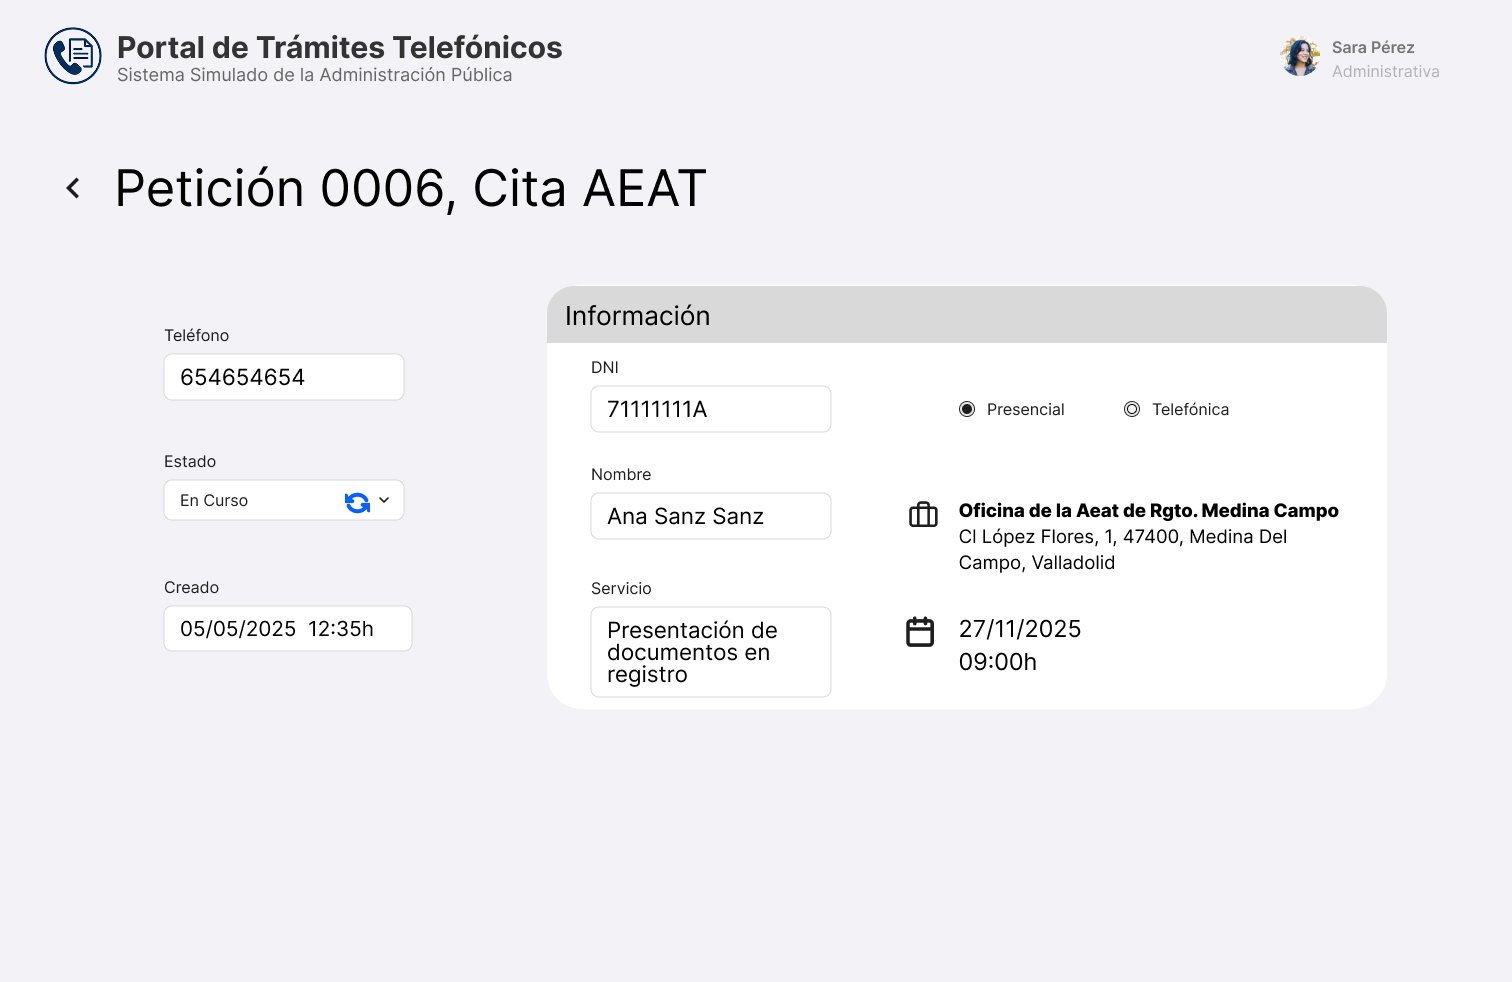
\includegraphics[width=0.8\textwidth]{img/mockups/Peticion.png}
        \caption{Prototipo visual de la página con detalles de una petición.}
        \label{fig:4.3}
    \end{figure}
    \begin{figure}[H]
        \centering
        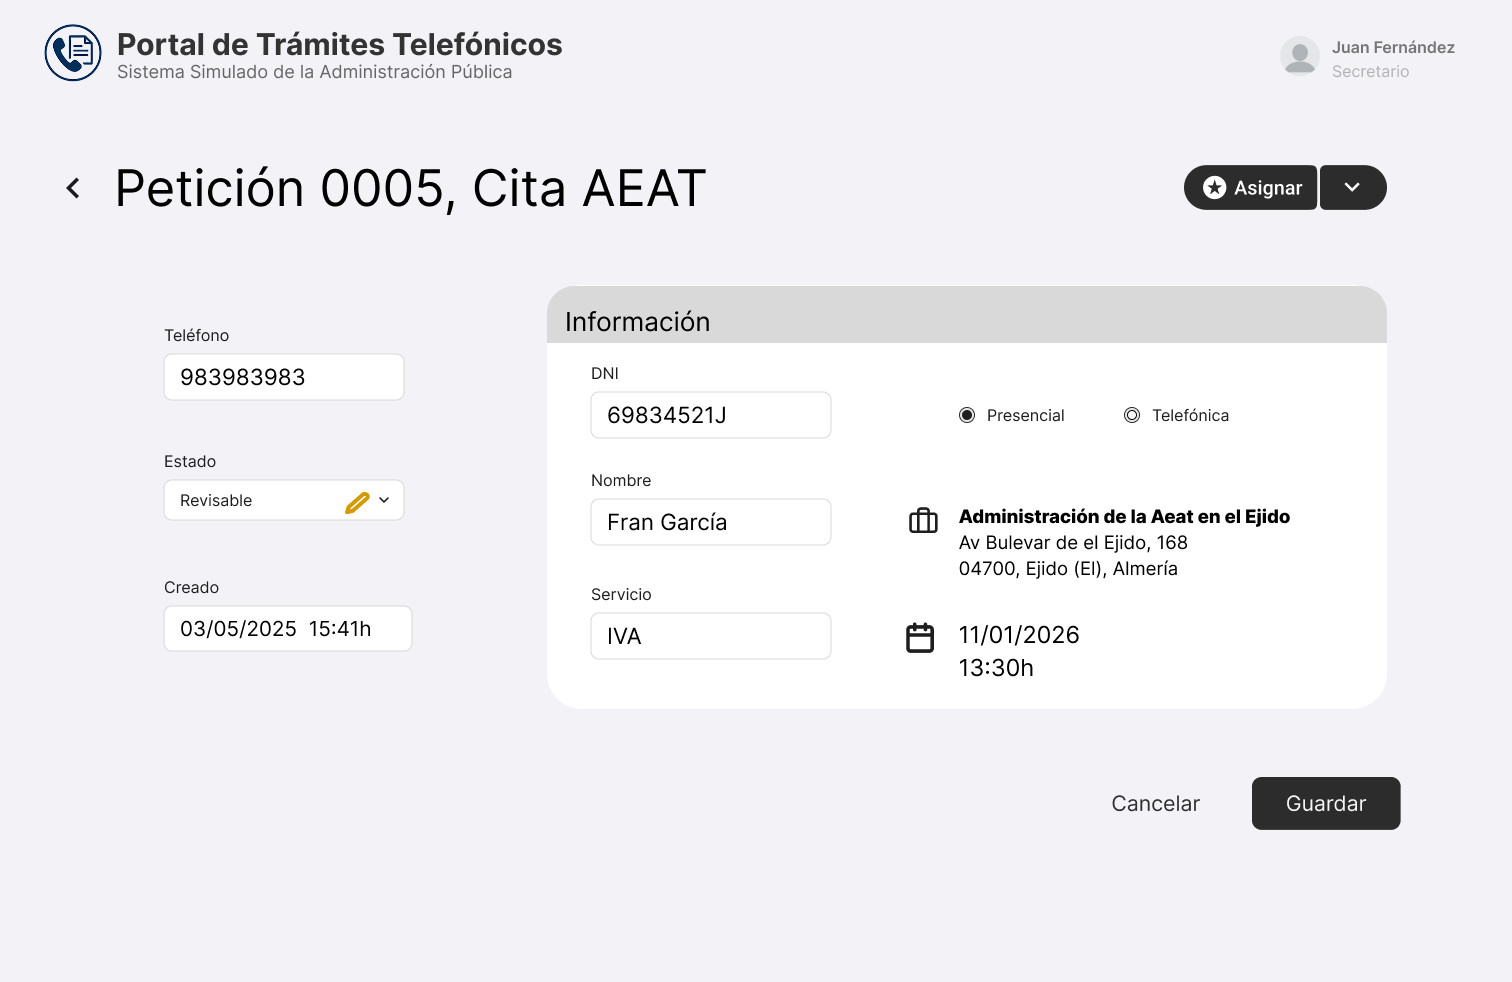
\includegraphics[width=0.8\textwidth]{img/mockups/Revisable.png}
        \caption{Prototipo visual de la página de una petición revisable.}
        \label{fig:4.4}
    \end{figure}
    Al clicar en el ID de una petición en la tabla de la imagen \ref{fig:4.2}, se muestra la página con detalles de la figura \ref{fig:4.3}.
    En esta pantalla se podrá consultar los datos concretos de una petición para cada trámite. 
        
    En caso de ser una petición revisable, figura \ref{fig:4.4}, los empleados que tengan permiso, verán a la derecha del título de la petición un botón para asignársela.
    Una vez asignada, los campos con la información se volverán modificables y los trabajadores podrán editar la petición o cancelarla.
        
    \begin{figure}[H]
        \centering
        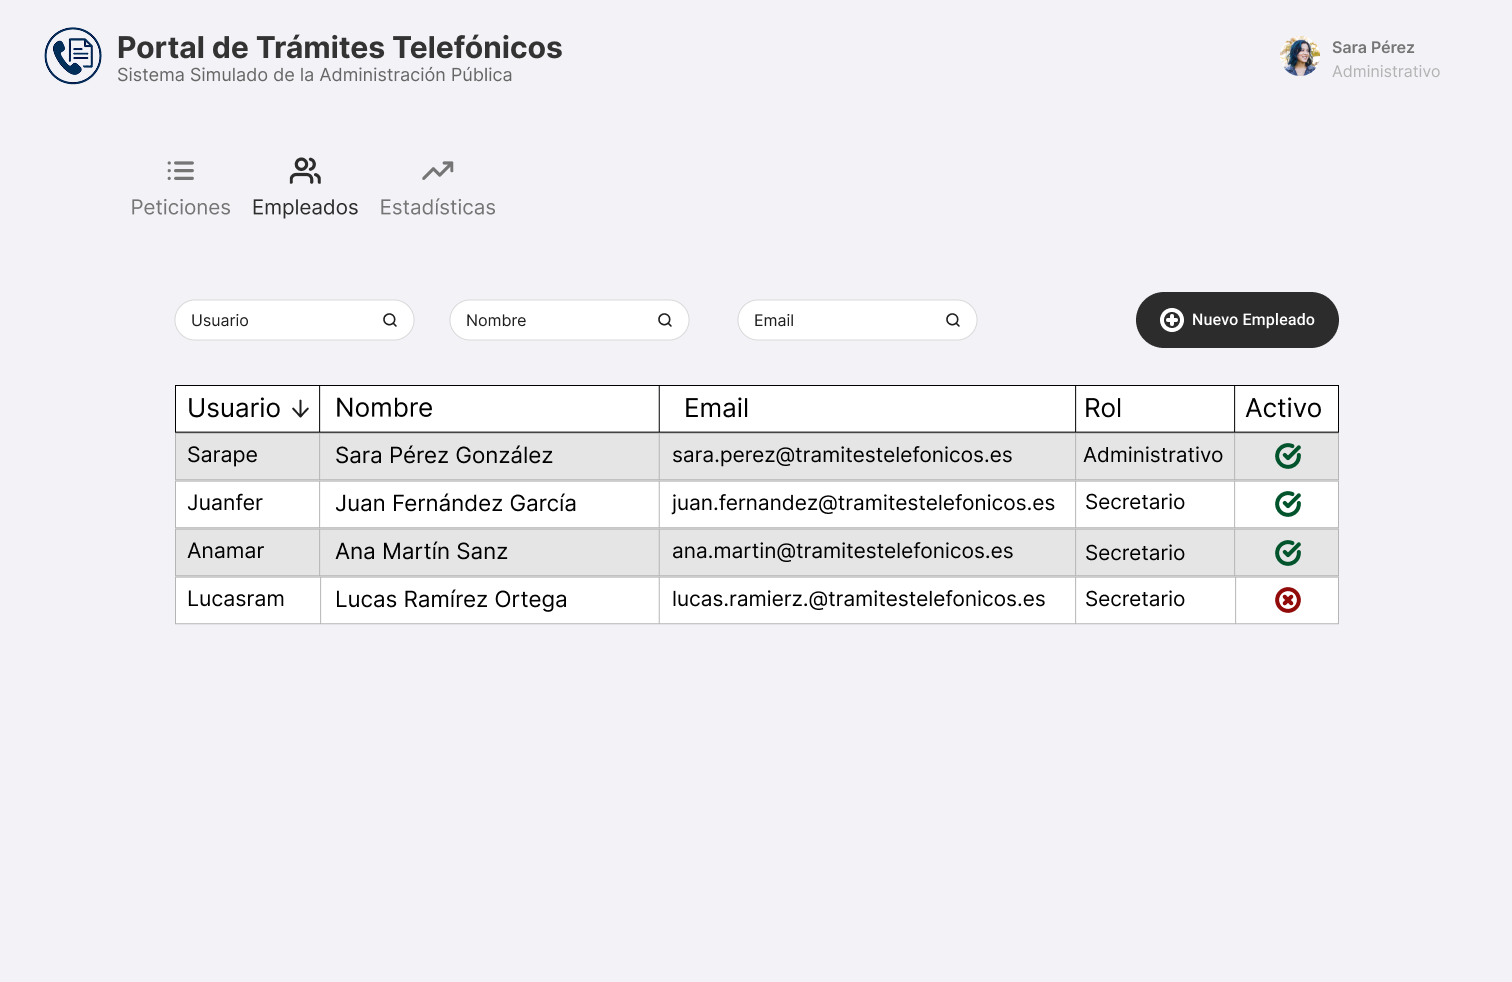
\includegraphics[width=0.8\textwidth]{img/mockups/Empleados.png}
        \caption{Prototipo visual de la página de empleados.}
        \label{fig:4.5}
    \end{figure}
    Desde el menú superior, los administradores pueden navegar hasta la figura \ref{fig:4.5}, que muestra un listado con todos los empleados del sistema. 
    El componente principal es una tabla similar a la de las peticiones, que incluye la información de cada empleado y los filtros necesarios para localizarlos rápidamente.
        
    A diferencia de la otra tabla, se añade una columna que indica si la cuenta de cada empleado está activa. 
    Esta columna cumple una doble función, ya que, clicando sobre el valor correspondiente a un empleado, se navegará hasta una página donde se muestra su información, permitiendo modificarla.
        
    La posibilidad de desactivar cuentas impide el acceso al sistema de un empleado sin necesidad de eliminar su cuenta, perservando así la trazabilidad de la información.
        
    Por último, se incluye a la derecha de los filtros el botón para poder agregar nuevos empleados al sistema.
        
    La página que muestra la información de los trámites será exactamente igual a esta, manteniendo los mismos componenetes, disposición y funcionalidad.

    \begin{figure}[H]
        \centering
        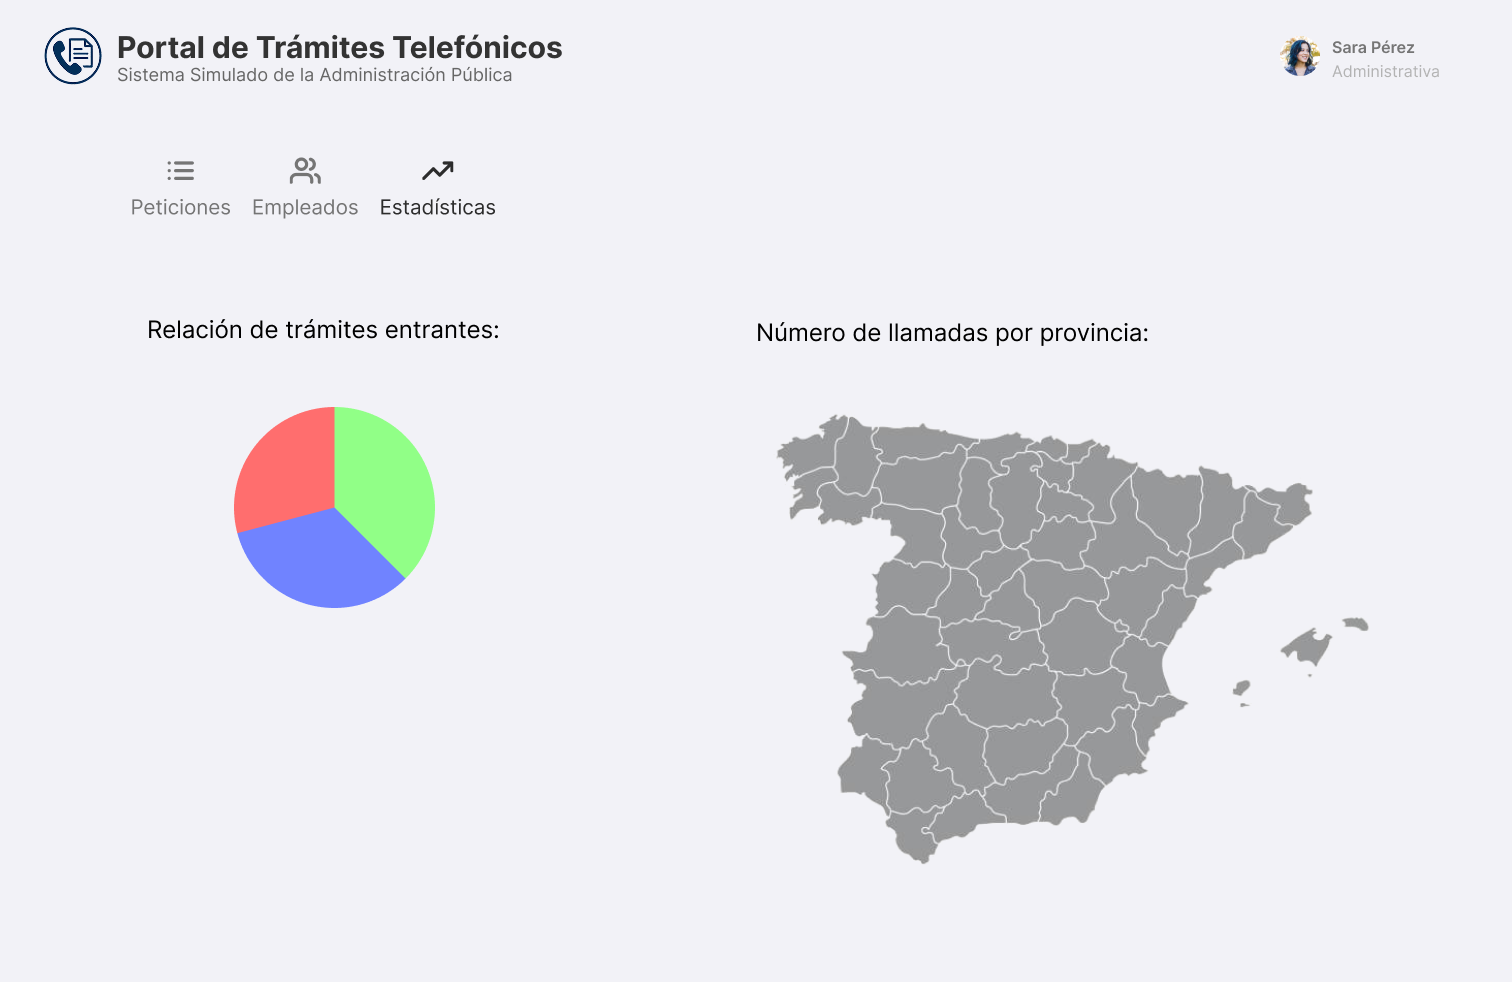
\includegraphics[width=0.8\textwidth]{img/mockups/Estadisticas.png}
        \caption{Prototipo visual de la página de estadísticas.}
        \label{fig:4.6}
    \end{figure}
    Desde el menú de navegación, también se puede acceder a una sección de estadísticas.
    Esta página está diseñada para mostrar información relevante sobre las peticiones y las llamadas recibidas.
    Dado que se trata de un sistema simulado, no habrá datos suficientes para que la información sea representativa. 
    Sin embargo, la sección queda incluida en el diseño como un desarrollo previsto a futuro.

\section{Arquitectura del sistema}
    La arquitectura principal del sistema se organiza como un modelo de capas relajadas, separando la funcionalidad en cuatro capas independientes. 
    Esta arquitectura implica que cada capa no se comunica únicamente con el nivel inmediatamente inferior, si no que habrá una capa superior que se comunique con las demás. 
    Esto se debe a que se ha adaptado la arquitectura al framework de Flask, por ello, el sistema no sigue un patrón modelo-vista-controlador estricto. 
        
    La capa principal es la capa de presentación, que incluye las vistas de la aplicación web y los controladores. 
    Flask funciona con rutas que se definen con una función, por lo que cada controlador puede incluir múltiples rutes. 
    Es decir, se usan controladores ligeros ya que cada controlador puede gestionar múltiples vistas. 
    Y al ser un sistema moderno, desde los mismos controladores se comunican con las otras tres capas, lo que implica que no puedan ser estrictas.

    La capa de negocio incluye únicamente un archivo desde el que se controlan los permisos de los empleados. 
    El resto de la lógica de negocio está definida implícitamente en las rutas. 

    En la capa de persistencia, se incluyen únicamente los modelos ORM, ya que sirven para representar la estructura de las entidades de la base de datos y encapsular su acceso. 
    Con esta herramienta, no es necesario crear un singleton propio para la conexión con la base de datos, ya que esa funcionalidad ya viene incluida.

    Por último, hay una capa de servicios que incluye los archivos del sistema que se utilizan para comunicarse con los servicios externos a la aplicación. 
    Principalmente, se usan las prestaciones de Google Cloud y Discord, aunque también incluye el servicio de correo interno y los procesos de automatización para ejecutar los trámites en las webs oficiales. 
        
    \begin{figure}[H]
        \centering
        
\includegraphics[width=0.8\textwidth]{img/diagramas/decomposition&uses_style.png}
        \caption{Decomposition \& Uses style.}
    \end{figure}

\section{Diseño de la base de datos}
    En esta sección se presenta el diseño de la base de datos del sistema, estructurada para almacenar toda la información necesaria para el correcto funcionamiento de la aplicación. 
    En la figura \ref{fig:4.8} se representa el diagrama entidad relación, siguiendo una representación fiel al modelo de dominio.
        
    \begin{figure}[H]
        \centering
        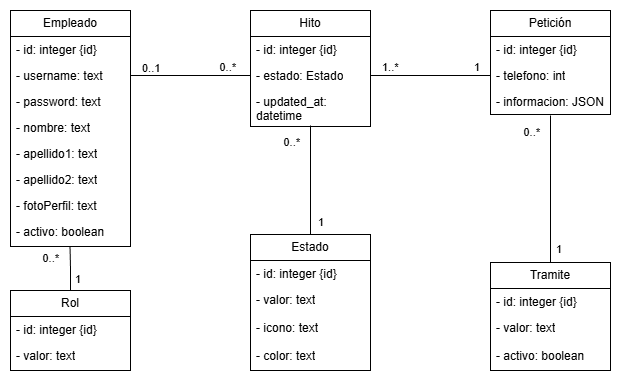
\includegraphics[width=1\textwidth]{img/diagramas/modelo_datos.png}
        \caption{Diagrama Entidad-Relación.}
        \label{fig:4.8}
    \end{figure}

\section{Diseño de la inteligencia artificial}
    El agente conversacional de Dialogflow funciona mediante la definición de intents y entities, implementando tecnologías de machine learning para detectar y analizar la intención que tiene el usuario. 
        
    Las posibles intenciones de los usarios se definen en los intents. 
    Se describen las frases de entrada o eventos que activan el intent, las contestaciones que debe dar el bot y las entities necesarias que se deben obtener. 
    Cuando el usuario dice una frase de entrada, la inteligencia artificial calcula la probabilidad de que coinicida con un intent, y si el porcentaje supera el umbral, activa la intención.
        
    Las entities sirven para definir los tipos de datos o la forma en la que se extrae la información de las frases.
    En otras palabras, sirven para categorizar o etiquetar las palabras. 
    Por ejemplo, "Quiero agendar una cita en la AEAT para mañana a las 10" podríamos extraer agendar una cita en la AEAT como una entidad de tipo trámite, mañana como fecha y las 10 como hora. 
    De esta forma también podemos saber que tipos de datos necesitamos al recopilar información, si un número, un texto, una dirección\dots
        
    Para la resolución de los trámites escogidos se han definido los siguientes intents: 
    \begin{itemize}
        \item Bienvenida: se activará automáticamente cuando el usuario inicia la llamada y activará un evento de espera de trámties.
        \item Tramite certificado empadronamiento, tramite cita AEAT y tramite tarjeta SACYL: se activarán cuando el usuario los solicite y el evento de espera de trámite esté activo y solicitarán los datos necesarios para cada trámite.
        \item Cita AEAT Modalidad: una vez recuperada la información inicial del tramite cita AEAT, se activa este intent desde el backend solo si el servicio escogido ofrece también cita telefónica.
        \item Cita AEAT Presencial: si el usuario solicita una cita presencial, el bot recupera la información correspondiente sobre la oficina y la fecha.
        \item Confirmar datos: una vez recuperada la información necesaria, se activará este intent para solicitar al usuario la vericidad de los datos y finalizar la llamada.
        \item Cambiar campo: en caso de que haya algún dato erróneo, se activará este intent para que el usuario pueda modificarlo.
    \end{itemize}

    También será necesario estipular los siguientes entities para facilitar la captura de la información: 
    \begin{itemize}
        \item Centros de salud de Valladolid: un enum con los centros de salud de Valladolid.
        \item DNI o pasaporte: una entidad regexp para limitar la variable al formato del DNI o pasaporte.
        \item Motivo tarjate SACYL: enum con los posibles motivos para solicitar la tarjeta.
        \item Municipios Valladolid: enum con todos los municipios de Valladolid.
        \item Oficina AEAT Valladolid: enum con las oficinas disponibles de la agencia tributaria en Valladolid.
        \item Servicios AEAT: un enum con la lista de servicios de la agencia tributaria.
        \item Teléfono: un variable regexp con el formato de los números telefónicos españoles.
        \item Tipo de cita: enum con los posibles tipos de cita en la AEAT.
        \item Trámite: enum con los trámites disponibles.
    \end{itemize}

    Por último, se ha definido en la figura \ref{fig:4.9} un digrama de flujo para definir la sescuencia prevista de una llamada al sistema.
    \begin{figure}[H]
        \centering
        
\includegraphics[width=0.8\textwidth]{img/diagramas/diagrama_flujo_ia.png}
        \caption{Diagrama de flujo del agente conversacional.}
        \label{fig:4.9}
    \end{figure}

\section{Seguridad y control de accesos}